
%%%%%%%%%%%%%%%%%%%%%%%%%%%%%%%%%%%%%%%%%
% Jacobs Landscape Poster
% LaTeX Template
% Version 1.1 (14/06/14)
%
% Created by:
% Computational Physics and Biophysics Group, Jacobs University
% https://teamwork.jacobs-university.de:8443/confluence/display/CoPandBiG/LaTeX+Poster
% 
% Further modified by:
% Nathaniel Johnston (nathaniel@njohnston.ca)
%
% This template has been downloaded from:
% http://www.LaTeXTemplates.com
%
% License:
% CC BY-NC-SA 3.0 (http://creativecommons.org/licenses/by-nc-sa/3.0/)
%
%%%%%%%%%%%%%%%%%%%%%%%%%%%%%%%%%%%%%%%%%

%----------------------------------------------------------------------------------------
%	PACKAGES AND OTHER DOCUMENT CONFIGURATIONS
%----------------------------------------------------------------------------------------

\documentclass[final]{beamer}

\usepackage[scale=1.24]{beamerposter} 					% Use the beamerposter package for laying out the poster
\usetheme{confposter} 								% Use the confposter theme supplied with this template

\setbeamercolor{block title}{fg=ngreen,bg=} 				% Colors of the block titles
\setbeamercolor{block body}{fg=black,bg=} 				% Colors of the body of blocks
\setbeamercolor{block alerted title}{fg=white,bg=dblue!70}		% Colors of the highlighted block titles
\setbeamercolor{block alerted body}{fg=black,bg=dblue!10}	% Colors of the body of highlighted blocks
\setbeamercolor{item}{fg=ngreen}						% Colors for itemize items
\setbeamercolor{item projected}{fg=white,bg=ngreen}		% Colors for enumerate items
\setbeamercolor{titlelike}{bg=green,fg=green}				% Color for title
\setbeamertemplate{items}[circle]						% Shape of enumerate 

\setbeamertemplate{background}{
\begin{tikzpicture}[remember picture,overlay]
		\path [top color = gray!10, middle color = gray!20, bottom color = gray!35] (current page.south west)rectangle (current page.north east);   % Adjust the position of the logo.
\end{tikzpicture}
}

% Many more colors are available for use in beamerthemeconfposter.sty

%-----------------------------------------------------------
% Define the column widths and overall poster size
% To set effective sepwid, onecolwid and twocolwid values, first choose how many columns you want and how much separation you want between columns
% In this template, the separation width chosen is 0.024 of the paper width and a 4-column layout
% onecolwid should therefore be (1-(# of columns+1)*sepwid)/# of columns e.g. (1-(4+1)*0.024)/4 = 0.22
% Set twocolwid to be (2*onecolwid)+sepwid = 0.464
% Set threecolwid to be (3*onecolwid)+2*sepwid = 0.708

\newlength{\sepwid}
\newlength{\onecolwid}
\newlength{\twocolwid}
\newlength{\threecolwid}
\setlength{\paperwidth}{48in} 			 % A0 width: 46.8in
\setlength{\paperheight}{36in} 			 % A0 height: 33.1in
\setlength{\sepwid}{0.024\paperwidth}	 % Separation width (white space) between columns
\setlength{\onecolwid}{0.22\paperwidth} 	 % Width of one column
\setlength{\twocolwid}{0.464\paperwidth}	 % Width of two columns
\setlength{\threecolwid}{0.708\paperwidth} % Width of three columns
\setlength{\topmargin}{-0.5in} 			 % Reduce the top margin size
%-----------------------------------------------------------

\usepackage{graphicx}  											% Required for including images
\usepackage{subfig}												% Required for formatting images close together.
\graphicspath{{"/Users/hgducharme/Programming/Undergraduate/RiceREU/Poster/Figures/"}}	% Location of the graphics files.
\usepackage{booktabs} 											% Top and bottom rules for table
\usepackage{verbatim}											% Used for multi-line comments
\usepackage[scaled=0.90]{helvet}									% Change font to Helvetica
\setbeamerfont{title}{family*=DejaVuSans}
\usefonttheme{professionalfonts}


%----------------------------------------------------------------------------------------
%	TITLE SECTION 
%----------------------------------------------------------------------------------------

\title{Asphaltene Deposition from Destabilized Oils with Water Emulsions Using Porous Microfluidics Chip} % Poster title

\author{Hunter Ducharme$^1$, Peng He$^2$, Yu-Jiun ``Nate'' Lin$^2$, Sibana Lisa Biswal$^2$} % Author(s)

\institute{$^1$ Rice Office of STEM Engagement, Rice University \\ 
	      $^2$ Chemical and Bimolecular Engineering, Rice University} % Institution(s)

%----------------------------------------------------------------------------------------

\begin{comment}
% Allows for pictures on left and right side of title by introducing three columns, instead of just one for the title
\setbeamertemplate{headline}{
 \leavevmode
  \begin{columns}
   \begin{column}{.2\linewidth}
    
\includegraphics[width=\linewidth]{logo.png}
   \end{column}
   \begin{column}{.6\linewidth}
    \vskip1cm
    \centering
    \usebeamercolor{title in headline}{\color{jblue}\Huge{\textbf{\inserttitle}}\\[0.5ex]}
    \usebeamercolor{author in headline}{\color{fg}\Large{\insertauthor}\\[1ex]}
    \usebeamercolor{institute in headline}{\color{fg}\large{\insertinstitute}\\[1ex]}
    \vskip1cm
   \end{column}
   \begin{column}{.2\linewidth}
    
\includegraphics[width=\linewidth]{logo.png}
   \end{column}
   \vspace{1cm}
  \end{columns}
 \vspace{0.5in}
 \hspace{0.5in}\begin{beamercolorbox}[wd=47in,colsep=0.15cm]{cboxb}\end{beamercolorbox}
 \vspace{0.1in}
}
\end{comment}

%----------------------------------------------------------------------------------------

\begin{document}

\addtobeamertemplate{block end}{}{\vspace*{2ex}} 		 % White space under blocks
\addtobeamertemplate{block alerted end}{}{\vspace*{2ex}} % White space under highlighted (alert) blocks

\setlength{\belowcaptionskip}{2ex}	  % White space under figures
\setlength\belowdisplayshortskip{2ex} % White space under equations

\begin{frame}[t, fragile] % The whole poster is enclosed in one beamer frame

\begin{columns}[t] % The whole poster consists of three major columns, the second of which is split into two columns twice - the [t] option aligns each column's content to the top

\begin{column}{\sepwid}\end{column} % Empty spacer column
\begin{column}{\onecolwid} 		 % The first column

%----------------------------------------------------------------------------------------
%	OBJECTIVES
%----------------------------------------------------------------------------------------

\begin{comment}
\begin{alertblock}{Objective}
To understand the effects of various salts on ashplatene deposition relating to water-in-oil emulsions.
\end{alertblock}
\end{comment}

%----------------------------------------------------------------------------------------
%	INTRODUCTION
%----------------------------------------------------------------------------------------

\begin{block}{Introduction}

\begin{itemize}
\item{\textcolor{ngreen}{\textbf{Asphaltenes}} are naturally found inside of crude oil that precipitate in the presence of a solvent, a change in pressure, and/or a change in temperature \cite{Kamran-Akbarzadeh:2007aa}.}
\item{\textcolor{ngreen}{\textbf{The problem is}} water emulsions increase the deposition of asphaltenes inside of flow lines and reservoir rocks \cite{Goual:2012aa}.}
\item{\textcolor{ngreen}{\textbf{The objective is}} to understand the effects of various salts on ashplatene deposition relating to water-in-oil emulsions.}
\end{itemize}

\end{block}

%---------------------------------------------------------------------

\begin{figure}
\fbox{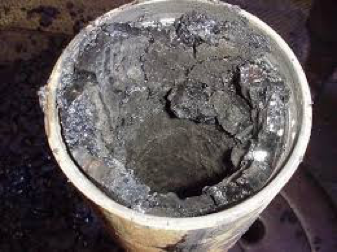
\includegraphics[width=0.45\linewidth]{clogged_pipe.png}}
\caption{Deposition of asphaltenes inside of a pipe. Andrews, A. (2006, September/October). [Clogged pipe]. Retrieved August, 2016.}
\end{figure}

%----------------------------------------------------------------------------------------
%	MATERIALS AND METHODS
%----------------------------------------------------------------------------------------

\begin{block}{Materials and Methods}

\begin{figure}
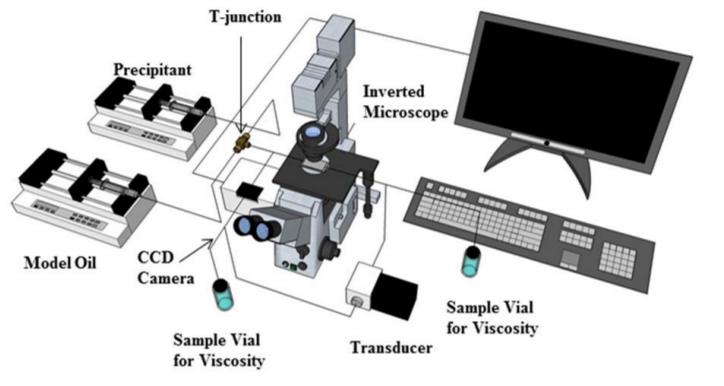
\includegraphics[width=0.9\linewidth]{materials.png}
\caption{Experimental setup. Courtesy of Yu-Jiun ``Nate'' Lin.}
\end{figure}

\begin{enumerate}
\item All materials are set up according to Figure 2.
\item Heptane and crude oil are pumped into the microfluidic device.
\item The pressure is recorded using a transducer.
\item Asphaltene deposition is recorded and measured using high speed optical microscopy.
\end{enumerate}

\end{block}

%---------------------------------------------------------------------

\end{column}						% End of the first column

\begin{column}{\sepwid}\end{column}	% Empty spacer column
\begin{column}{\twocolwid}			% Begin a column which is two columns wide (column 2)
\begin{columns}[t,totalwidth=\twocolwid]	% Split up the two columns wide column
\begin{column}{\onecolwid}\vspace{-.6in}	% The first column within column 2 (column 2.1)

%----------------------------------------------------------------------------------------
%	WATER'S IMPACT
%----------------------------------------------------------------------------------------

\begin{block}{Water's Impact on Deposition}

Increasing the presence of water in crude oil positively correlates with asphaltene deposition and the aggregation of emulsions.

\vspace{1em}

\begin{figure}[!tbp]
  \centering
  \subfloat{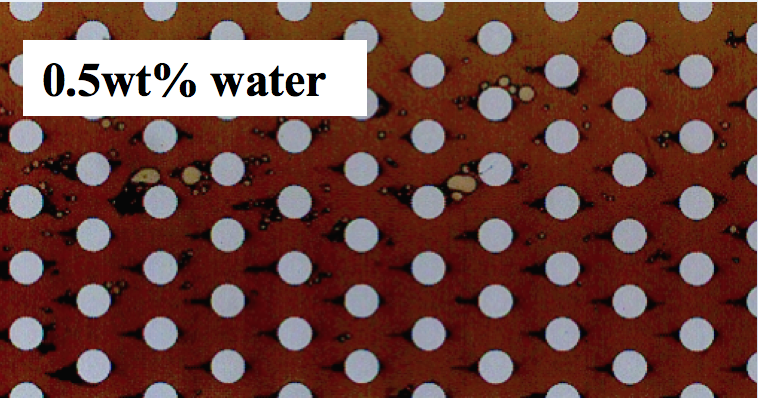
\includegraphics[width=0.49\textwidth]{05wt.png}}
  \hfill
  \subfloat{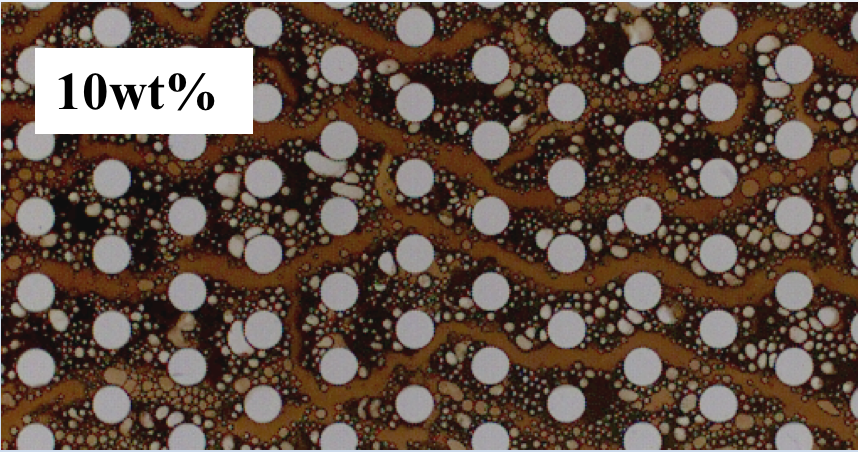
\includegraphics[width=0.49\textwidth]{10wt.png}} \\
  
  \subfloat{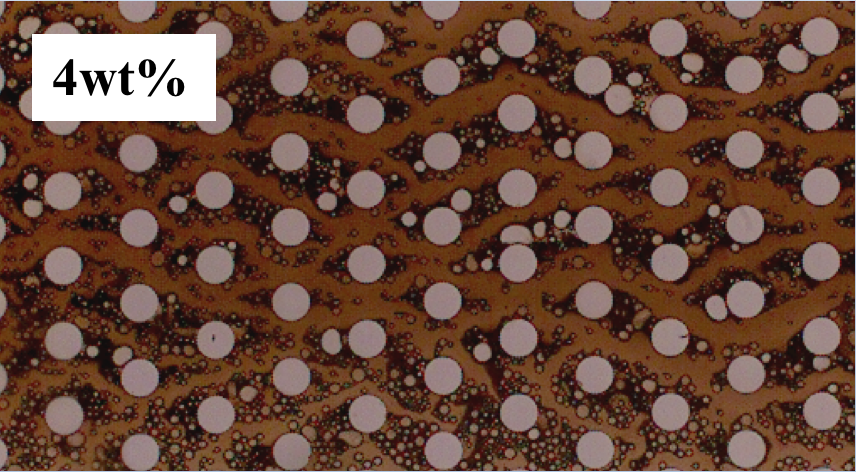
\includegraphics[width=0.49\textwidth]{4wt.png}}
  \hfill
  \subfloat{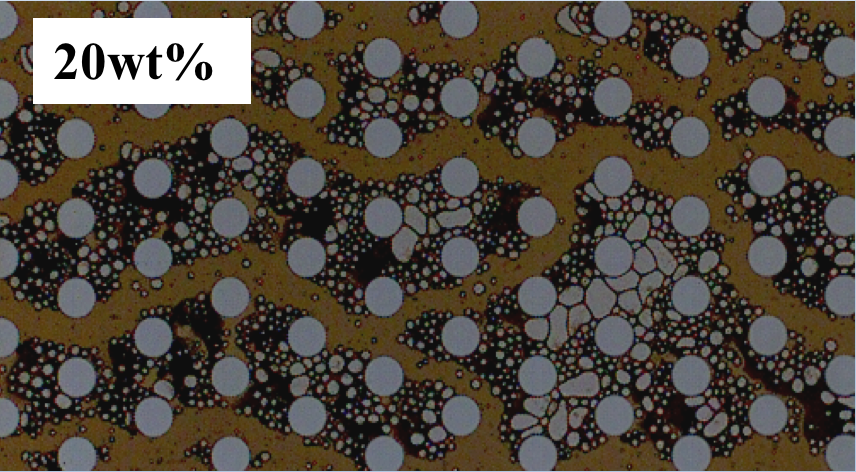
\includegraphics[width=0.49\textwidth]{20wt.png}}
  \caption{Asphaltene deposition inside the porous media with varying water concentrations. Courtesy of Yu-Jiun ``Nate'' Lin.}
\end{figure}

\vspace{0.5em}

\end{block}

%----------------------------------------------------------------------------------------

\end{column} % End of column 2.1

\begin{column}{\onecolwid}\vspace{-.6in} % The second column within column 2 (column 2.2)

%----------------------------------------------------------------------------------------
%	SALT'S EFFECT
%----------------------------------------------------------------------------------------

\begin{block}{Salt's Impact on Deposition}

\begin{figure}
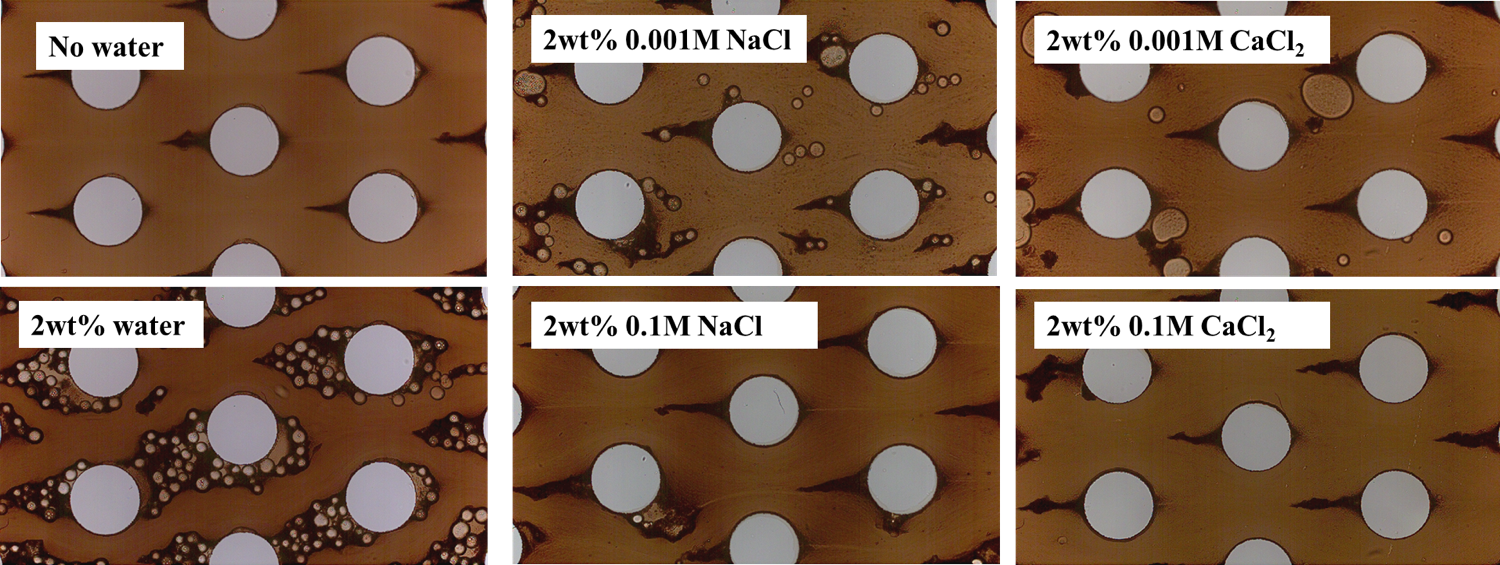
\includegraphics[width=0.8\linewidth]{salts.png}
\caption{Asphaltene deposition inside the porous media with 2\% of volume being water in addition to varying concentrations of sodium. Courtesy of Yu-Jiun ``Nate'' Lin.}
\end{figure}

Nunc tempus venenatis facilisis. Curabitur suscipit consequat eros non porttitor. Sed a massa dolor, id ornare enim:

\begin{figure}
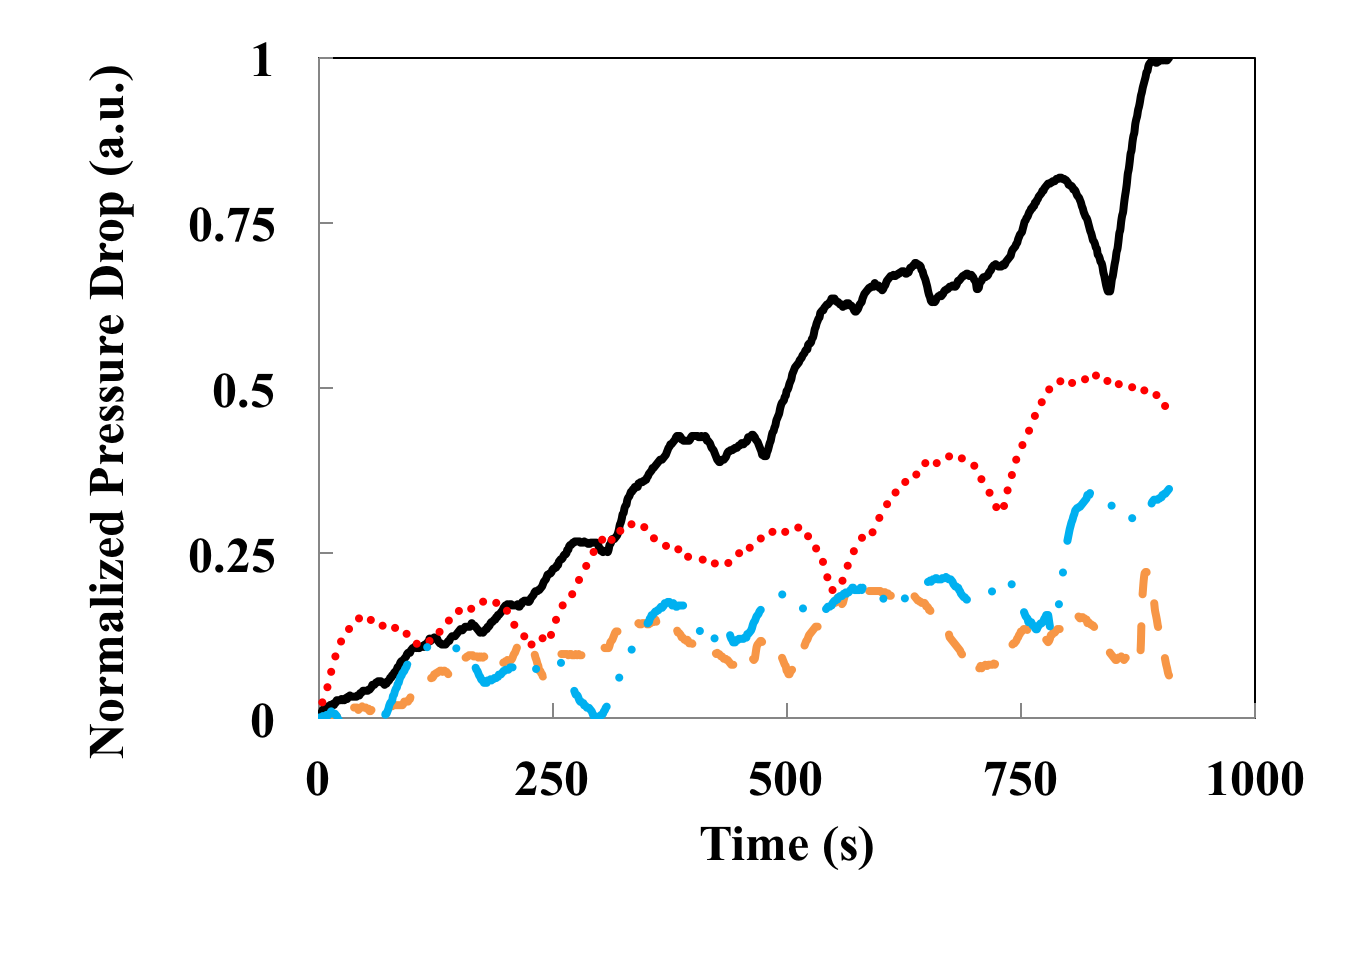
\includegraphics[width=0.9\linewidth]{2wt_salts.png}
\caption{Experimental setup. Courtesy of Yu-Jiun ``Nate'' Lin.}
\end{figure}

\begin{figure}
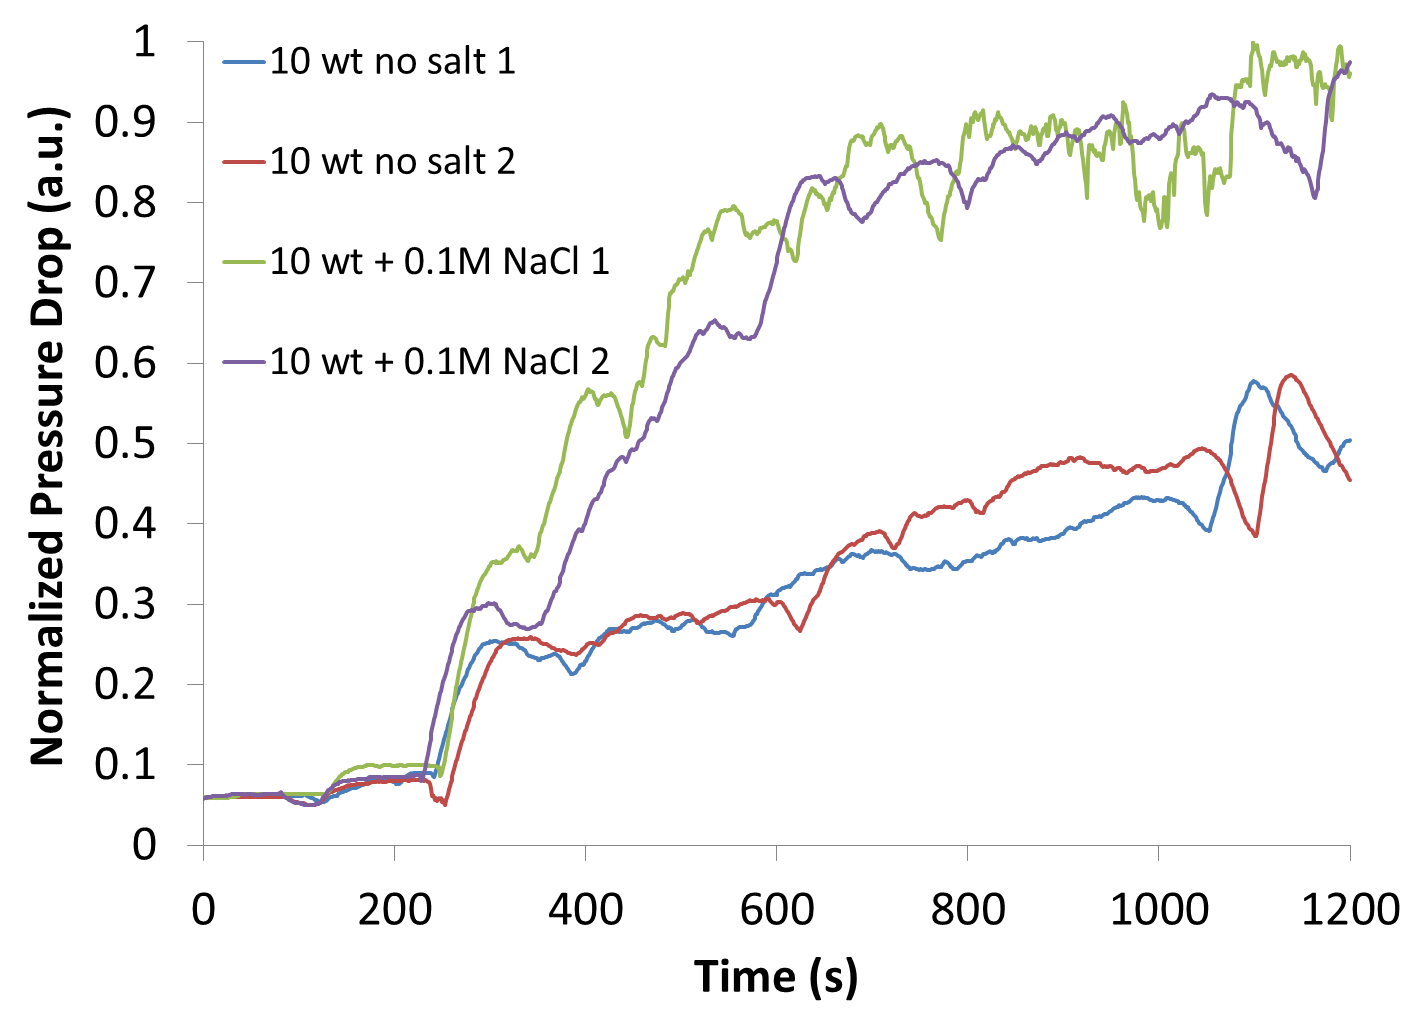
\includegraphics[width=0.9\linewidth]{10wt_salts.png}
\caption{Experimental setup. Courtesy of Yu-Jiun ``Nate'' Lin.}
\end{figure}

\end{block}

%----------------------------------------------------------------------------------------

\end{column}	% End of column 2.2
\end{columns}	% End of the split of column 2 - any content after this will now take up 2 columns width
\end{column}	% End of the second column

\begin{column}{\sepwid}\end{column} % Empty spacer column
\begin{column}{\onecolwid} 		 % The third column

%----------------------------------------------------------------------------------------
%	CONCLUSION
%----------------------------------------------------------------------------------------

\begin{block}{Conclusion}

\begin{itemize}
\item Nunc tempus venenatis facilisis. 
\item \textbf{Curabitur suscipit} consequat eros non porttitor. 
\item Sed a massa dolor, id ornare enim. 
\end{itemize}

\end{block}

\begin{comment}
%----------------------------------------------------------------------------------------
%	ADDITIONAL INFORMATION
%----------------------------------------------------------------------------------------

\begin{block}{Additional Information}

Maecenas ultricies feugiat velit non mattis. Fusce tempus arcu id ligula varius dictum. 
\begin{itemize}
\item Curabitur pellentesque dignissim
\item Eu facilisis est tempus quis
\item Duis porta consequat lorem
\end{itemize}

\end{block}
\end{comment}

%----------------------------------------------------------------------------------------
%	REFERENCES
%----------------------------------------------------------------------------------------

\begin{block}{References}

\nocite{*} % Insert publications even if they are not cited in the poster
\small{\bibliographystyle{unsrt}
\bibliography{sample}}

\end{block}

%----------------------------------------------------------------------------------------
%	CONTACT INFORMATION
%----------------------------------------------------------------------------------------

% \setbeamercolor{block alerted title}{fg=black,bg=norange} % Change the alert block title colors
% \setbeamercolor{block alerted body}{fg=black,bg=white} % Change the alert block body colors

\begin{block}{Contact Information}

\begin{itemize}
\item Email: hgducharme@gmail.com
\item Phone: 281-450-7154
\end{itemize}

\end{block}

\begin{center}
\begin{tabular}{ccc}

\includegraphics[width=0.4\linewidth]{logo.png} & \hfill & 
\includegraphics[width=0.4\linewidth]{logo.png}
\end{tabular}
\end{center}

%----------------------------------------------------------------------------------------

\end{column} % End of the third column

\end{columns} % End of all the columns in the poster

\end{frame}
\end{document}
